\chapter{Relativité sans gravité}

    La notion de relativité consiste en l'existence d'un ensemble de référentiels, dits \textit{référentiels inertiels} dans lesquels les lois de la physique prennent la même forme. Les transformations permettant de passer d'un référentiel à un autre sont des \textit{symétries} des lois de la physique et l'ensemble de ces transformations forment un \textit{groupe de symétries} (ou \textit{groupe de relativité}).

    \section{Relativité galiléenne}
    
        Si l'on dispose d'un premier système de coordonnées $(\vv{x},t)$, alors les trois transformations élémentaires en relativité galiléenne permettant de passer à un deuxième système de coordonnées $(\vv{x}',t')$ et laissant les lois de la physique invariantes sont
        \begin{itemize}[label = \textbullet]
            \item les translations spatiales : $\vv{x}' = \vv{x}+\vv{a}$ avec $a\in\mathbb{R}^3$
            \item les rotations spatiales : $\vv{x}' = \mathcal{R}(\vv{x})$ avec $x'^a = R^a_{~b}x^b,~R\in SO(3)$
            \item les translations temporelles : $t' = t + t_0$ avec $t_0\in\mathbb{R}$
        \end{itemize}
        
        \begin{rmk}
            Le fait que l'on utilise des vecteurs en physique est une conséquence de l'invariance par rotation des lois de la physique et non l'inverse. C'est d'ailleurs ce qui différencie un vecteur d'un triplet de nombres : les lois de transformation des composantes d'un vecteur sous changement de base sont bien précises (transformation linéaire sous le groupe de symétrie), alors qu'un triplet de nombre n'a aucune propriété de ce type qui lui est imposée a priori.
        \end{rmk}
        
        \begin{definition}
            Si le référentiel $(\vv{x}',t')$ est vu comme se déplaçant à une vitesse $\vv{v}$ dans le référentiel $(\vv{x},t)$ alors la \textit{transformation de Galilée} permet de passer de $(x,t)$ à $(\vv{x}',t')$ comme suit:
            \begin{subequations}\label{TSL}
            \begin{empheq}[left=\empheqlbrace]{align}
                \vv{x}' &= \vv{x}-\vv{v}t \\
                t' &= t
            \end{empheq}
            \end{subequations}
        \end{definition}
        
        \begin{prin}[de relativité]
        \begin{leftbar}
            Tous les référentiels galiléens sont équivalents pour décrire les lois fondamentales de la nature. Elles conservent leur forme pour tout changement de référentiel galiléen.
        \end{leftbar}
        \end{prin}
    
    \section{Relativité einsteinienne}
    
        \subsection{Constance de la vitesse de la lumière}
    
            Le principe de relativité est toujours présent mais on y ajoute un second principe.
            
            \begin{prin}[constance de la vitesse de la lumière]
            \begin{leftbar}
                Dans le vide, la lumière se propage toujours avec une certaine vitesse $c$ qui est indépendante de l'état de mouvement de la source lumineuse. Cela peut se traduire par le fait que la vitesse de la lumière dans le vide est une constante indépendante du référentiel d'observation.
            \end{leftbar}
            \end{prin}
            
            La relativité einsteinienne est un bond conceptuel par rapport à la relativité galiléenne car elle mélange les coordonnées de temps et d'espace (temps relatif). Les transformations qui laissent les lois de la physique invariantes sont les mêmes mais les transformations qui permettent de passer d'un référentiel à un autre ne sont plus les transformations de Galilée mais les \textit{transformations de Poincaré}.\\
            
		\subsection{Espace-temps de Minkowski et groupe de Poincaré}            
            
            Avant de définir le groupe de symétrie (groupe de Poincaré), commençons par définir l'espace-temps de cette relativité. Après cela, nous définirons un sous-groupe du groupe de Poincaré qui a une importance capitale.
            
            \begin{definition}
                L'\textit{espace-temps de Minkowski} (ou \textit{espace-temps de Poincaré-Minkowski}) est l'espace euclidien à quatre dimension $\mathbb{R}^4$ munit de la pseudo-métrique de Minkowski $\eta$ de signature $(-,+,+,+)$.
            \end{definition}
            
            Le produit scalaire entre $v^\alpha = (v^0,\vv{v})$ et $w^\alpha = (w^0,\vv{w})$ est alors définit comme
            \begin{equation}
                v\cdot w = \eta_{\alpha\beta}v^\alpha w^\beta = v_\alpha w^\alpha = -v^0w^0+\vv{v}\cdot\vv{w}.
            \end{equation}
            La norme induite par ce produit scalaire n'est pas définie positive :
            \begin{equation}
            \norm{v}^2 = v\cdot v = \eta_{\alpha\beta}v^\alpha v^\beta = v_\alpha v^\alpha = -(v^0)^2+\vv{v}^2.
            \end{equation}
            C'est pour cela que l'on parle de pseudo-norme et de pseudo-métrique.
            
            \begin{definition}
                On appelle \textit{évènement} de coordonnées $x^\mu$ et on note $\underline{x}$, un point de coordonnées $(x^0,x^1,x^2,x^3)$ dans l'espace-temps. On dit que $x^\mu$ est la \textit{quadri-position} de cet évènement.
            \end{definition}
            
            Un évènement peut désigner n'importe quelle action considérée comme instantanée: l'émission d'un signal lumineux, la désintégration d'une particule, ... Comme pour n'importe quel espace vectoriel normé, la norme découle du produit scalaire. Dans notre cas, la pseudo-métrique est dite hyperbolique ce qui a des conséquences bien particulières que nous verrons dans la suite.\\
            
            On peut maintenant définir le groupe formé par l'ensemble des transformations linéaires qui agissent sur les coordonnées et qui préservent la métrique de Minkowski (isométries).
            \begin{definition}
                Le \textit{groupe de Lorentz} (ou \textit{groupe de Lorentz homogène}) est défini comme
                $$O(3,1)~\hat{=}~\left\{\Lambda\in M_{4\times 4}(\mathbb{R})~\big|~\Lambda^T\eta\Lambda = \eta\right\}$$
            \end{definition}
            
			\begin{definition}
				Soit $v=(v^0,\vv{v})\in\mathbb{R}^4$, on dit que $v^\mu$ est un \textit{quadri-vecteur} s'il se transforme linéairement comme
				\begin{equation}
					v^\alpha\to v'^\alpha = \Lambda^\alpha_{~\beta}v^\beta
				\end{equation}
				sous la transformation de Lorentz $\Lambda\in O(3,1)$.
			\end{definition}            
            En particulier, la quadri-position est un quadri-vecteur. Le produit scalaire et la norme que nous avons définit pour la quadri-position sont définis pour n'importe quel quadri-vecteur. On voit facilement que les transformations de Lorentz sont des isométries :
            \begin{equation}
                v\cdot w = \eta_{\alpha\beta}v^\alpha w^\beta = \eta_{\alpha\beta} \Lambda^\alpha_{~\delta}  \Lambda^\beta_{~\omega} v'^\delta w'^\omega = \eta_{\delta\omega}  v'^\delta w'^\omega = v'\cdot w'
            \end{equation}
            
            La relativité einsteinienne est une extension de la relativité galiléenne donc elle est également invariante sous les translations spatiales et temporelles. Si l'on ajoute ces transformations au groupe de Lorentz, on obtient le groupe de symétrie de la relativité einsteinienne : le groupe de Poincaré.
            \begin{definition}
                Le \textit{groupe de Poincaré} $ISO(3,1)$ est le groupe formé par le groupe de Lorentz, les translations dans le temps et les translations dans l'espace.
                \begin{equation}
                    ISO(3,1) ~\hat{=}~ \mathbb{R}^{3,1}\rtimes O(3,1)
                \end{equation}
                Ce groupe est parfois appelé \textit{groupe de Lorentz affine} ou \textit{groupe de Lorentz inhomogène}.
            \end{definition}
            
            Ce groupe agit sur les coordonnée de l'espace-temps comme
            \begin{equation}
                x'^\alpha = \Lambda^\alpha_{~\beta}x^\beta + a^\mu
            \end{equation}
            avec $\Lambda\in O(3,1)$ et $a\in\mathbb{R}^4$. C'est un groupe non-abélien à 10 paramètres.
            
            \begin{rmk}
                Soient deux transformations $(\Lambda_1,a_1),(\Lambda_2,a_2)\in ISO(3,1)$. Si l'on applique la première transformation sur un quadri-vecteur quelconque $x$ on obtient
                \begin{equation}
                	x' = \Lambda_1x+a_1.
                \end{equation}
                En apppliquat la seconde transformation au résultat, on obtient
                \begin{equation}
                x'' = \Lambda_2x'+a_2 = \Lambda_2\Lambda_1x+\Lambda_2a_1+a_2
                \end{equation}
                donc $(\Lambda_2,a_2)\circ(\Lambda_1,a_1) = (\Lambda_2\Lambda_1,\Lambda_2a_1+a_2)$. Cette règle particulière pour le produit ne correspond pas à celle d'un produit direct mais bien à celle d'un produit semi-direct.
            \end{rmk}
            
            Le groupe de Lorentz est un sous-groupe du groupe de Poincaré qui a une importance capitale. Il parfois lui-même présenté comme le groupe de symétrie de la relativité restreinte car il contient les transformations les plus intéressantes conceptuellement. Le sous-groupe $\mathbb{R}^4$ des translations dans l'espace-temps est déjà présent en relativité galiléenne.
            
            \begin{prop}\begin{leftbar}
                Le groupe de Lorentz possède quatre composantes connexes:
                \begin{align}
                    L^\uparrow_+ &~\hat{=}~ \left\{\Lambda\in O(3,1)~\big|~\text{det}(\Lambda) = 1\text{ et }\Lambda^0_{~0}\geq1\right\} \\
                    L^\downarrow_+ &~\hat{=}~ \left\{\Lambda\in O(3,1)~\big|~\text{det}(\Lambda) = 1\text{ et }\Lambda^0_{~0}\leq -1\right\} \\
                    L^\uparrow_- &~\hat{=}~ \left\{\Lambda\in O(3,1)~\big|~\text{det}(\Lambda) = -1\text{ et }\Lambda^0_{~0}\geq1\right\} \\
                    L^\downarrow_- &~\hat{=}~ \left\{\Lambda\in O(3,1)~\big|~\text{det}(\Lambda) = -1\text{ et }\Lambda^0_{~0}\leq-1\right\}
                \end{align}
                où les signes $+,-$ donnent le signe du déterminant et les flèches $\uparrow,\downarrow$ donnent le sens du temps.
            \end{leftbar}\end{prop}
            
            \begin{proof}
            ${}$\\
                Soit $\Lambda\in O(3,1)$, alors
                \begin{equation}
                    -1 = \det(\eta) = \det(\Lambda^T\eta\Lambda) = -\det(\Lambda)^2
                \end{equation}
                donc $\det(\Lambda) = \pm 1$. De plus, en prenant la composante $00$ de l'égalité $\eta = \Lambda^T\eta\Lambda$ on obtient
                \begin{equation}
                    -1 = \eta_{00} = \Lambda^\mu_{~0}\eta_{\mu\nu}\Lambda^\nu_{~0} = -(\Lambda^0_{~0})^2+\sum_{a=1}^3(\Lambda^a_{~0})^2.
                \end{equation}
                Il n'y a donc que deux possibilités pour $\Lambda^0_{~0}$ :
                \begin{equation}
                    \Lambda^0_{~0} \geq 1 \text{\quad ou \quad} \Lambda^0_{~0} \leq -1.
                \end{equation}
                Donc, quel que soit $\Lambda\in O(3,1)$, $\Lambda$ appartient à un et un seul des quatre ensembles définis ci-dessus. Montrons que chaque ensemble est connexe. On fait le raisonnement pour $L_+^\uparrow$, les autres étant similaires.\\
                Soient $\Lambda_1, \Lambda_2 \in L_+^\uparrow$ et $\Lambda(t)$ une courbe continue telle que $\Lambda(t) = \Lambda_1 (1 - t) + t\Lambda_2, ~\forall t \in [0,1]$. Dans ce cas, 
                \begin{align}
                    \det \Lambda(t) &= (1 - t)\det \Lambda_1 + t \det \Lambda_2 = (1 - t) + t = 1\\
                    \Lambda^0_{~0}(t) &= (1 - t)(\Lambda_1)^{0}_{~0} + t(\Lambda_2)^{0}_{~0} \ge (1 - t) + t = 1
                \end{align}
                et donc $\Lambda(t) \in L_+^\uparrow~\forall t \in [0,1]$, ce qui dit exactement que $L_+^\uparrow$ est connexe. \\
                De plus,  
                \begin{equation}
                    O(3, 1) = L_+^\uparrow \cup L_+^\downarrow \cup L_-^\uparrow \cup L_-^\downarrow 
                \end{equation}
                et comme ces quatre ensembles sont disjoints et connexes, nous avons bien montré la décomposition de $O(3, 1)$ en ses quatre composantes connexes.\\
                Notons que cette décomposition est unique. En effet, supposons qu'il existe une composante connexe $L \subset O(3, 1)$. Comme l'union de nos quatre composantes recouvrent $O(3, 1)$, il existe un $L^i_j$ ($i = ~\uparrow, \downarrow$ et $j = +, -$) tel que 
                \begin{equation}
                    L \cap L^i_j \neq \varnothing
                \end{equation}
                Soient $\Lambda \in L \cap L^i_j $ et $\Lambda' \in L\backslash L^i_j$. Dans ce cas, il existe un $L^k_l \neq L^i_j$ tel que $\Lambda' \in L^k_l$. Par connexité de $L$, il existe une courbe $\Lambda(t)$ continue telle que $\Lambda(0) = \Lambda$ et $\Lambda(1) = \Lambda'$
                ce qui contredit le fait de $L$ et $L'$ sont des composantes connexes distinctes.
                %ce qui est absurde car on ne peut pas passer continûment de $\Lambda^0_{~0} \geq 1$ à $\Lambda^0_{~0} \leq -1$ ou de $\det \Lambda = 1$ à $\det \Lambda = -1$. 
                Donc $L$ est nécessairement une des quatre composantes explicitées.
            \end{proof}
            \begin{definition}
                On dit qu'une transformation de Lorentz est \textit{propre} (\textit{impropre}) si $\text{det}(\Lambda) = 1$ ($\det(\Lambda) = -1$) et \textit{orthochrone} (\textit{non-orthochrone}) si $\Lambda^0_{~0}\geq1$ ($\Lambda^0_{~0}\leq-1$). 
            \end{definition}
            Notons que parmi les quatre composantes connexes du groupe de Lorentz, seul la composante $L^\uparrow_+$ (transformations de Lorentz propres orthochrones) est un groupe car c'est la seule à contenir l'identité. De plus, c'est un sous-groupe normal.
            
            \begin{definition}
                Le \textit{groupe de Lorentz propre} est défini comme
                $$SO(3,1) ~\hat{=}~ \left\{\Lambda\in O(3,1)~\big|~\text{det}(\Lambda) = 1\right\} = L^\uparrow_+\cup L^\downarrow_+.$$
                On le note aussi $L_+$. Le \textit{groupe de Lorentz propre orthochrone} est défini comme
                $$L^\uparrow_+ ~\hat{=}~ \left\{\Lambda\in SO(3,1)~\big|~\Lambda^0_{~0}\geq1\right\}.$$
            \end{definition}
            
            \begin{prop}\begin{leftbar}
                Le groupe de Lorentz est formé par les transformations de Lorentz propres orthochrones, le renversement du temps $T$ ($t\to -t$) et la parité $P$ ($\vv{x}\to -\vv{x}$).
            \end{leftbar}\end{prop}
            \begin{proof}${}$\\
                \comp
            \end{proof}
            
            Étant donné que le renversement du temps $T$ et la parité $P$ permettent de passer de $L^\uparrow_+$ aux autres composantes connexes, l'essentiel se trouve dans $L^\uparrow_+$. Ce groupe contient les transformations spéciales de Lorentz et les rotations statiques de l'espace. Nous allons voir que ce groupe est composé des rotations et d'autres transformations de Lorentz appelées transformations spéciales de Lorentz.
            
            \begin{definition}
                Si le référentiel $(\vv{x}',t')$ est vu comme se déplaçant à une vitesse $v\in]-1,1[$ selon l'axe des $x$ dans le référentiel $(\vv{x},t)$ alors la \textit{transformation spéciale de Lorentz}  (\textit{T.S.L.} ou \textit{boost}) de $(\vv{x},t)$ à $(\vv{x}',t')$ a la forme
                \begin{subequations}\label{TSL}
                \begin{empheq}[left=\empheqlbrace]{align}
                    t' &= \gamma(v)(t-vx), \\
                    x' &= \gamma(v)(x-vt), \\
                    y' &= y, \\
                    z' &= z,
                \end{empheq}
                \end{subequations}
                où $\gamma(v)=\frac{1}{\sqrt{1-v^2}}$.
            \end{definition}
            Ces transformations peuvent également s'écrire sous forme matricielle comme
            \begin{equation}
            	\begin{bmatrix}
            		t'\\
            		x'\\
            		y'\\
            		z'
            	\end{bmatrix}=
            	\begin{bmatrix}
            		\gamma & -\gamma\beta & 0 & 0 \\
            		-\gamma\beta & \gamma & 0 & 0 \\
            		0 & 0 & 0 & 0 \\
            		0 & 0 & 0 & 0
            	\end{bmatrix}
            	\begin{bmatrix}
            		t\\
            		x\\
            		y\\
            		z
            	\end{bmatrix}
            \end{equation}
            où $\beta=\frac{v}{c}$ dans les unités CKM.
            
            \begin{rmk}
            	Les T.S.L. forment un groupe à un paramètre.
            \end{rmk}
            \begin{rmk}
                Nous avons défini les transformations spéciales de Lorentz directement par une forme explicite qui semble venir de nulle part. Nous verrons après qu'il existe plusieurs manières de trouver l'expression des transformations de Lorentz dont certaines ne font même pas référence à la lumière. Par exemple dans \cite{leblond}, il est démontré que l'on peut trouver la forme explicite des transformations de Lorentz juste à partir des quatre hypothèses suivantes : homogénéité de l'espace-temps, isotropie de l'espace-temps, l'ensemble des changements de référentiels possède une structure de groupe et le principe de causalité.
            \end{rmk}
            
            \begin{prop}\begin{leftbar}
                Toute transformation de Lorentz propre orthochrone $\Lambda\in L^\uparrow_+$ peut être décomposée de manière unique comme le produit d'une rotation statique $R\in(1\oplus SO(3))$ et d'une T.S.L. $L(v)$.
                \begin{equation}
                    \Lambda = RL
                \end{equation}
            \end{leftbar}\end{prop}
            
            \begin{proof}${}$\\
                \comp                
            \end{proof}
            
            \begin{prop}\begin{leftbar}
                Les groupes $O(3)$ et $SO(3)$ peuvent être vus comme des sous-groupes (par isomorphisme) de $L_+^\uparrow$ comme
                \begin{align}
                    \{\Lambda\in L_+^\uparrow|\Lambda^0_{~0}&=1\}\simeq O(3)\\
                    \{\Lambda\in L_+^\uparrow|\Lambda^0_{~0}&=1 \text{ et } det(\Lambda)=1\}\simeq SO(3).
                \end{align}
            \end{leftbar}\end{prop}
            
            \begin{proof}${}$\\
                \comp
            \end{proof}
            
            \begin{figure}[H]
            \centering
            \begin{tikzpicture}
                \node (O) at (2,3.464) {$O(3, 1)$};
                \node (Lp) at (0,0) {$L_+ = SO(3,1)$};
                \node (Lm) at (4,0) {$L_-$};    
                \node (Lpu) at  (-1,-1.732) {$L_+^\uparrow$};
                \node (Lpd) at  (1,-1.732) {$L_+^\downarrow$};
                \node (Lmu) at  (3,-1.732) {$L_-^\uparrow$};
                \node (Lmd) at  (5,-1.732) {$L_-^\downarrow$};
                \node (S) at  (-2,-3.464) {$1 \oplus SO(3)$};
                \node (T) at  (0,-3.464) {T.S.L.};
                \node (RC) at  (4,4.5) {$\mathbb{R}^{3,1} \rtimes O(3, 1)$};
                \node (R) at  (6,3.464) {$\mathbb{R}^{3,1}$};
                \tikzstyle{estun}=[->, >=latex]
                \draw[estun] (O)--(Lp); \draw[estun] (O)--(Lm);
                \draw[estun] (Lp)--(Lpu); \draw[estun] (Lp)--(Lpd);
                \draw[estun] (Lm)--(Lmu); \draw[estun] (Lm)--(Lmd);
                \draw[estun] (Lpu)--(S); \draw[estun] (Lpu)--(T);
                \draw[estun] (RC)--(O); \draw[estun] (RC)--(R);
                \draw[<->, >=latex] (Lp) to[bend left] (Lm);
                \draw[<->, >=latex] (Lpu) to[bend left] (Lpd);
                \draw[<->, >=latex] (Lmu) to[bend left] (Lmd);
                \draw (0, -1.732) node{$T$};
                \draw (4, -1.732) node{$T$};
                \draw (2, 1) node{$P$};
            \end{tikzpicture}
            \caption{Représentation schématique de la structure du groupe de Poincaré}
            \end{figure}
            
            Le système \ref{TSL} donne la forme explicite d'une transformation de Lorentz spéciale de Lorentz lorsque $\vv{v}$ est selon l'axe des $x$. On voudrait trouver une forme pour $\vv{v}$ quelconque.
            
            \begin{prop}\begin{leftbar}
                Pour $\vv{v}$ quelconque, les transformations spéciales de Lorentz imposent le changement de coordonnées suivant:
                \begin{subequations}\label{TSLg}
                \begin{empheq}[left=\empheqlbrace]{align}
                t' &= \gamma(t-\vv{x}\cdot\vv{x},) \\
                \vv{x}' &= \vv{x} - \gamma t\vv{v} + (\gamma-1)\frac{\vv{x}\cdot\vv{v}}{\vv{v}^2}\vv{v}.
                \end{empheq}
                \end{subequations}
            \end{leftbar}\end{prop}
            
            \begin{proof}
            ${}$\\
            Une première méthode, basée sur l'intuition, permet de trouver un résultat rapidement. Soient $\vv{F}(t,\vv{x},\vv{v})$ et $\vv{G}(t,\vv{x},\vv{v})$ deux fonctions inconnues telles que
            \begin{subequations}
                \begin{empheq}[left=\empheqlbrace]{align}
                    t' &= \vv{F}(t,\vv{x},\vv{v}) \\
                    \vv{x}' &= \vv{G}(t,\vv{x},\vv{v})
                \end{empheq}
            \end{subequations}
            Il n'y a qu'une seule manière de combiner $\vv{v}$ et $\vv{x}$ pour que $t'$ satisfasse \ref{TSL} :
            \begin{equation}
                t' = \gamma(t-\vv{v}\cdot\vv{x}).
            \end{equation}
            Pour $\vv{x}'$, si l'on veut pouvoir retrouver la limite galiléenne, il faut que $\vv{G}$ soit linéaire en $\vv{x}$ et $\vv{v}$, donc
            \begin{equation}
                \vv{x}' = A\vv{x} + B\vv{v}
            \end{equation}
            où les coefficients $A$ et $B$ peuvent dépendre de la norme de $\vv{v}$ et du temps. Lorsque $\vv{v}=(v,0,0)$ il faut que $y'=y$ et $z'=z$. En faisant le même raisonnement avec $\vv{v}$ selon les autres axes de coordonnée spatiale, on déduit que $A = 1$.\\
            Toujours dans le cas $\vv{v}=(v,0,0)$, nous avons alors
            \begin{equation}
                x' = x+Bv = \gamma(x-vt)
            \end{equation}
            et donc $B = (\gamma-1)\frac{x}{v}-\gamma t$. Le terme $\frac{x}{v}$ devient $\frac{\vv{x}\cdot\vv{v}}{\vv{v}\cdot\vv{v}}$ lorsque $\vv{v}$ est quelconque.\\
            
            Le deuxième méthode est plus calculatoire. Il suffit d'appliquer la matrice $R$ de rotation de $x$ à $\vv{v}$ quelconque à la matrice $\lambda$. C'est faire un changement de base
            
            \begin{equation}
                \begin{pmatrix}
                aa
                \end{pmatrix}
            \end{equation}
            \comp
            \end{proof}
            
            Nous avons vu comment faire pour trouver la forme la plus générale des T.S.L. à partir du cas $\vv{v} = (v,0,0)$, mais comment faire pour trouver la forme de cette dernière dans un premier temps ? Il existe plusieurs manières de trouver la forme des transformations de Lorentz. Une des manières les plus courantes est d'imposer l'invariance de la vitesse de la lumière en faisant un changement de référentiel. En supposant que le temps ne soit pas absolu, on trouve alors la manière dont se dilatent les intervalles de temps et le reste en découle. Cette façon de procéder a l'avantage d'être simple et intuitive mais donne l'impression que la relativité restreinte concerne principalement la lumière, ce qui est faux. La relativité restreinte concerne toute la cinématique en physique. Le terme "restreint" désignant cette théorie est donc assez mal choisi étant donné qu'elle est indépendante de l'interaction considérée et est de ce fait plus générale que la relativité "générale" qui est une théorie de la gravitation. Ce nom a été historiquement donné pour désigner le fait qu'elle ne comprenait pas la gravitation, ce qui la rend paradoxalement beaucoup plus générale.
            
            \begin{definition}
                On appelle \textit{intervalle d'espace-temps} entre deux évènements $P_1$ et $P_2$ respectivement de coordonnées $x_1^\mu$ et $x_2^\mu$ la quantité
                \begin{align}
                    \underline{P_1P_2}^2&~\hat{=}~ \eta_{\alpha\beta}(x_2^\alpha-x_1^\alpha)(x_2^\beta-x_1^\beta) \\
                    &= \underline{P_1P_2}\cdot\underline{P_1P_2} \\
                    &= -x_1^0 x_2^0 + x_1^1 x_2^1 + x_1^2 x_2^2 + x_1^3 x_2^3.
                \end{align}
                $$$$
                On dit que l'intervalle est 
                \begin{itemize}[label = \textbullet]
                    \item de \textit{genre temps} si $\underline{P_1P_2}^2<0$
                    \item de \textit{genre lumière} si $\underline{P_1P_2}^2=0$
                    \item de \textit{genre espace} si $\underline{P_1P_2}^2>0$
                \end{itemize}
            \end{definition}
            
            \begin{prop}\begin{leftbar}
                Soient deux évènements $P_1$ et $P_2$ respectivement de coordonnées $x_1^\mu$ et $x_2^\mu$ et l'intervalle d'espace-temps $\underline{u}^2 = \eta_{\mu\nu}x_1^\mu x_2^\nu$.
                \begin{itemize}[label = \textbullet]
                    \item Si $\underline{u}^2<0$, il existe un référentiel pour lequel les évènements $P_1$ et $P_2$ sont au même point de l'espace à des instants différents, c'est-à-dire qu'il existe une transformation de Lorentz $\Lambda$ telle que
                    \begin{equation}
                        \underline{u}' = \Lambda \underline{u} = \left(u'^0,\vv{0}\right).
                    \end{equation}
                    Donc $P_1$ et $P_2$ sont liés causalement.
                    \item Si $\underline{u}^2>0$, il existe un référentiel pour lequel les évènements $P_1$ et $P_2$ se trouvent à des endroits distincts de l'espace au même moment, c'est-à-dire qu'il existe une transformation de Lorentz $\Lambda$ telle que
                    \begin{equation}
                        \underline{u}' = \Lambda \underline{u} = \left(0,\vv{u'}\right).
                    \end{equation}
                    Donc $P_1$ et $P_2$ ne sont pas liés causalement.
                    \item Si $\underline{u}^2=0$, il existe un référentiel pour lequel les évènements $P_1$ et $P_2$ sont liés par un signal lumineux, c'est-à-dire qu'il existe une transformation de Lorentz $\Lambda$ telle que
                    \begin{equation}
                        \underline{u}' = \Lambda \underline{u} = \left(u'^0,u'^0,0,0\right).
                    \end{equation}
                    Donc $P_1$ et $P_2$ sont liés causalement uniquement pas un champ électro-magnétique.
                \end{itemize}
            \end{leftbar}\end{prop}
            
            \begin{proof}${}$\\
                \comp
            \end{proof}
        
        \subsection{Quadri-vitesse et quadri-impulsion}
        
            Nous voudrions maintenant définir une notion de vitesse. Une première idée pourrait être de simplement dériver la position en fonction du temps $t$.
            \begin{definition}
                On appelle \textit{vitesse ordinaire} la quantité
                \begin{equation}
                v^\mu ~\hat{=}~ \frac{dx^\mu}{dt} = (1,\vv{v})
                \end{equation}
            \end{definition}
            Mais cette quantité n'est pas un quadri-vecteur. De manière générale, un tenseur dérivé par un scalaire (invariant) donne toujours un vecteur mais ici nous avons
            \begin{equation}
                dt = \gamma d\tau
            \end{equation}
            où $\tau$ est le temps propre. Donc $t$ n'est pas un scalaire de Lorentz : il se transforme sous les boosts. Ceci implique que 
            \begin{equation}
                v^\mu v_\mu = 1-v^2 
            \end{equation}
            n'est pas un invariant de Lorentz.\\
            Cependant, nous voyons que
            \begin{equation}
                v^\mu = \frac{dx^\mu}{dt} = \gamma \frac{dx^\mu}{d\tau}.
            \end{equation}
            et comme $\tau$ est un scalaire, $\frac{dx^\mu}{d\tau}$ est un quadri-vecteur.
            \begin{definition}
                On appelle \textit{quadri-vitesse} le quadri-vecteur
                \begin{equation}
                    U^\alpha(\tau) ~\hat{=}~ \frac{dx^\alpha}{d\tau}.
                \end{equation}
            \end{definition}
            La quadri-vitesse d'un objet ponctuel est donc définie comme étant la tangente à sa ligne d'univers. On peut montrer par développement direct que 
            \begin{equation}
                U^\alpha(\tau) = (\gamma,\gamma\vv{v})
            \end{equation}
            et que 
            \begin{equation}
                U_\alpha U^\alpha = \gamma^2\vv{v}^2-\gamma^2 = -1
            \end{equation}
        
            Soient deux référentiels $\mathcal{R}_1$ et $\mathcal{R}_2$ respectivement associés aux coordonnées $(t,\vv{x})$ et $(t',\vv{x}')$. Les vitesses dans chacun des référentiels sont définies comme
            \begin{align}
                \vv{v}_{\R_1} &= \frac{d\vv{x}}{dt} \\
                \vv{v}_{\R_2} &= \frac{d\vv{x}'}{dt}
            \end{align}
            
            \begin{prop}\begin{leftbar}
                Nous avons la loi de composition des vitesses suivante.
                \begin{equation}
                    \vv{v}_{\R_1} = \frac{\vv{v}_{\R_2}+\gamma\vv{v}+(\gamma-1)\frac{\vv{v}_{\R_2}\cdot\vv{v}}{\vv{v}^2}\vv{v}}{\gamma(1+\vv{v}\cdot\vv{v}_{\R_2})}
                \end{equation}
                où $\vv{v}$ est la vitesse de $\mathcal{R}_2$ dans $\mathcal{R}_1$.
            \end{leftbar}\end{prop}
            
            \begin{proof}
            ${}$\\
                Si l'on prend la transformation \ref{TSLg} avec $\vv{v} = \vv{v}_{\nicefrac{2}{1}}$, et que l'on inverse les relations, on obtient
                \begin{subequations}
                \begin{empheq}[left=\empheqlbrace]{align}
                    t &= \gamma(t'+\vv{x}'\cdot\vv{x}') \\
                    \vv{x} &= \vv{x}' + \gamma t'\vv{v} + (\gamma-1)\frac{\vv{x}'\cdot\vv{v}}{\vv{v}^2}\vv{v}
                \end{empheq}
                \end{subequations}
                Le système inverse peut être obtenu simplement en prenant $-\vv{v}$ à la place de $\vv{v}$. \\
                Et donc,
                \begin{align}
                    \vv{v}_{\R_1} &= \frac{d\vv{x}'+\gamma\vv{v}dt'+(\gamma-1)\frac{d\vv{x}'\cdot\vv{x}'}{\vv{v}^2}}{\gamma(dt'+\vv{v}\cdot d\vv{x}')}\\
                    &= \frac{\vv{v}_{\R_1}+\gamma\vv{v}+(\gamma-1)\frac{\vv{v}_{\R_1}\cdot\vv{v}}{\vv{v}^2}\vv{v}}{\gamma(1+\vv{v}\cdot\vv{v}_{\R_2})}
                \end{align}
            \end{proof}
            
            En particulier, si $\vv{v} = (v,0,0)$, 
            \begin{equation}
                v_{\R_1}  = \frac{v_{\R_2}+v_{\nicefrac{\R_2}{\R_1}}}{1+v_{\R_2}v_{\nicefrac{\R_2}{\R_1}}}.
                \label{LTVx}
            \end{equation}
            Ce résultat est à divisé par $c^2$ si l'on veut revenir au SI. Dans la limite classique, $\vv{v}_{\R_1},\vv{v}_{\R_2}\ll 1$ donc 
            \begin{equation}
             	v_{\R_1}  \approx v_{\R_2}+v_{\nicefrac{\R_2}{\R_1}}.
            \end{equation}
            
            La loi de composition des vitesses (\ref{LTVx}) n'est pas très compliquée mais elle peut être encore plus simple pour une paramétrisation de la vitesse bien choisie.
            
            \begin{definition}
                La \textit{rapidité} $\varphi$ est définie par
                \begin{equation}
                    v~\hat{=}~\th{\varphi}.
                \end{equation}
            \end{definition}
            
            La fonction tangente hyperbolique 
            $$\text{th}:\mathbb{R}\to~ ]-1,1[$$ 
            est une bijection donc cette paramétrisation a du sens.
            
            \begin{figure}[H]
    			\centering
    			\begin{tikzpicture}[scale=1.5]
        			\draw[->] (-3,0) -- (3,0)  node[below]{$\phi$};
        			\draw[->] (0,-2) -- (0,2) node[left]{$v$};
        			\draw[dashed] (-3,-1.5) -- (3,-1.5);
        			\draw[dashed] (-3,1.5) -- (3,1.5);
        			\draw[scale=1, domain=-3:3, smooth, variable=\x, blue]  plot ({\x}, {1.5*(e^\x-e^(-\x))/(e^\x+e^(-\x))});
    			\end{tikzpicture}
    			\caption{Rapidité en fonction de la vitesse}
    			\label{fig:my_label}
			\end{figure}
            
            
            
            \begin{prop}\begin{leftbar}
                La loi de transformation des vitesses pour la rapidité est linéaire et 
                \begin{equation}
                    \varphi_{\R_1} = \varphi_{\R_2}+\varphi_{\nicefrac{\R_2}{\R_1}}.
                \end{equation}
            \end{leftbar}\end{prop}
            
            \begin{proof}
            ${}$\\
                En supposant que $\vv{v} = (v,0,0)$, on pose $v_{\R_1} ~\hat{=}~ \th{\varphi_{\R_1})},~ v_{\R_2} ~\hat{=}~ \th{\varphi_{\R_2}}$ et $v_{\nicefrac{2}{1}} ~\hat{=}~ \th{\varphi_{\nicefrac{\R_2}{\R_2}}}$, la loi de transformation \ref{LTVx} devient
                \begin{equation}
                    \th{\varphi_{\R_1}} = \frac{\th{\varphi_{\R_2}}+\th{\varphi_{\nicefrac{\R_2}{\R_1}}}}{1+\th{\varphi_{\R_2}}\th{\varphi_{\nicefrac{\R_2}{\R_1}}}} = \th{\varphi_{\R_2}+\varphi_{\nicefrac{\R_2}{\R_1}}}
                \end{equation}
                donc on trouve bien
                \begin{equation}
                    \varphi_{\R_1} = \varphi_{\R_2}+\varphi_{\nicefrac{\R_2}{\R_1}}.
                \end{equation}
            \end{proof}
            
            La dernière proposition montre bien que la condition $v\leq 1$ qui est souvent placée au centre la relativité einsteinienne n'est pas tellement fondamentale. Cette condition provient uniquement de notre paramétrisation de la vitesse.\\
            
            Une mauvaise interprétation de la condition $v\leq1$ (et donc $v\leq c$ dans les unités MKS) peut aussi amener à croire que la distance maximale que l'on peut parcourir en un temps $\Delta t'$ est plus petite ou égale à $c\Delta t'$, ce qui est faux (cela dépend de l'objet qui se déplace). Un observateur peut se rendre n'importe où en n'importe quel temps. Par exemple, il est possible de se rendre à l'autre bout de la galaxie en une seconde et ceci n'est pas en contradiction avec $v\leq 1$. L'observateur qui se rend à l'autre bout de la galaxie ne se voit pas aller à une vitesse plus grande que $c$ par rapport aux planètes qu'il croise. Disons qu'il veut parcourir une distance $L$ vue par un observateur extérieur qui est dans le même référentiel que la galaxie, l'observateur qui se déplace dans la galaxie ne se voit pas parcourir une distance $L$ mais plutôt une distance $L' = L\sqrt{1-v^2}\leq L$ où $v$ est la vitesse de son référentiel par rapport au référentiel de la galaxie. Donc il se voit aller à une vitesse
            \begin{equation}
                \frac{L'}{\Delta t'} = \frac{L}{\Delta t'} \sqrt{1-v^2} = \sqrt{1-v^2}.
            \end{equation}
            \comp
            
            Dans le référentiel de la galaxie, l'observateur qui se déplace n'est pas non plus vu comme allant à une vitesse supra-luminique à cause la dilatation du temps.
            \begin{definition}
                On appelle \textit{quadri-impulsion} (ou \textit{énergie-impulsion}) le quadri-vecteur 
                \begin{equation}
                    P^\alpha = mU^\alpha
                \end{equation}
                où $m$ est la masse de l'objet considéré.
            \end{definition}
            En développant, on trouve que
            \begin{equation}
                P^\alpha = m U^\alpha = (\gamma m,\gamma m\vv{v}) = (E,\vv{p}).
            \end{equation}
            Ce quadri-vecteur est appelé énergie impulsion car sa partie spatiale correspond à l'impulsion classique multipliée par $\gamma$ (la partie spatiale correspond en fait à la quantité de mouvement mais on l'appelle souvent impulsion par anglicisme). La première composante est appelée \textit{énergie relativiste} et le second \textit{impulsion relativiste}. Dans le cas non-relativiste ($v\ll 1$), on retrouve bien
            \begin{align}
            	p^0 &= m+\frac{1}{2}mv^2,\\
            	\vv{p} &= m\vv{v}.
            \end{align}
La composante spatiale correspond donc à l'énergie au repos plus l'énergie cinétique et la partie spatiale correspond à la quantité de mouvement newtonnienne.
            
            \begin{rmk}
                L'énergie d'une masse ponctuelle de masse $m$ est donnée par
                \begin{equation}
                    E = \gamma m = \frac{m}{\sqrt{1-v^2}}
                \end{equation}
                et n'est donc pas bornée supérieurement. Il est possible d'ajouter un postulat à la relativité restreinte pour que ca soit le cas, c'est la \textit{relativité doublement restreinte}. Nous n'en parlerons pas dans ce cours.
            \end{rmk}
            
            \begin{prop}\begin{leftbar}
                Nous avons l'égalité suivante:
                \begin{equation}
                    E^2 = \vv{p}^2 + m^2.
                \end{equation}
            \end{leftbar}\end{prop}
            \begin{proof}
            ${}$\\
                Il suffit de développer l'expression de la norme de la quadri-impulsion.
                \begin{equation}
                P_\alpha P^\alpha = \vv{p}^2-E^2 = m^2\vv{v}^2\gamma^2-m^2\gamma^2 = -m^2
            \end{equation}
            \end{proof}
            
            Notons que la démonstration précédente implique bien que la masse (propre) est un invariant de Lorentz.\\
            
            Lorsque $\vv{p} = \vv{0}$, on obtient la célèbre équation
            \begin{equation}
                E = m.
            \end{equation}
            Dans les unités MKS : $E=mc^2$.
            
            En mécanique classique, l'énergie et l'impulsion d'un système isolé sont conservées. Ceci est indépendant du principe de relativité. La relativité restreinte donne des nouvelles valeurs à l'énergie et à l'impulsion mais ces grandeurs restent conservées au sein d'un même référentiel.\\
            
            \begin{prin}[conservation de l'énergie impulsion]
            \begin{leftbar}
                Pour tout système isolé, l'énergie-impulsion totale est conservée au cours du temps.
            \end{leftbar}
            \end{prin}
            
        \subsection{Quadri-accélération}
        
            En dérivant à nouveau par rapport au temps propre $\tau$, on peut introduire un nouveau quadri-vecteur correspondant cette fois à l'accélération.
            \begin{definition}
                On appelle \textit{quadri-accélération} le quadri-vecteur
                \begin{equation}
                    A^\alpha ~\hat{=}~ \frac{d^2x^\alpha}{d\tau^2}.
                \end{equation}
            \end{definition}
            On peut montrer par un développement direct que, à $1+1$ dimensions,
            \begin{equation}
                A^\alpha = \frac{d^2x^\alpha}{d\tau^2} = \frac{dU^\alpha}{d\tau} = \gamma\frac{dU^\alpha}{dt} = \left( \frac{v}{(1-v^2)^{\frac{5}{2}}}\frac{dv}{dt}, \frac{v^2}{(1-v^2)^{\frac{5}{2}}}\frac{dv}{dt} +\gamma \frac{dv}{dt}\right)
            \end{equation}
        
            Tout en considérant des référentiels inertiels, rien n'empêche de considérer des objets qui accélèrent dans ces référentiels. Pour simplifier les calculs qui suivent, on considère le cas où les mouvements se font uniquement selon $x$. Le mouvement uniformément accéléré est défini en relativité einsteinienne comme la ligne d'univers telle qu'un observateur qui la suivrait ressente une accélération constante.
            
            \begin{definition}
                On appelle \textit{accélération propre}, l'accélération dans le référentiel tangent à la ligne d'univers d'un mouvement uniformément accéléré, c'est-à-dire le référentiel dans lequel l'observateur est immobile à l'instant considéré.
            \end{definition}
            Autrement dit, l'accélération propre est l'accélération ressentie par l'observateur.
            \begin{rmk}
				Nous discuterons la cas de la gravitation plus tard mais on peu d'ores et déjà préciser qu'un observateur en chute libre ne ressent aucune accélération. Son accélération propre est nulle.
			\end{rmk}
             Supposons qu'un observateur en MRUA suive la trajectoire $(t(\tau),x(\tau))$ où $\tau$ est le temps propre, vu d'un référentiel $\mathcal{R}$ fixe de coordonnées $(t,x)$. A chaque instant $\tau$, on a un référentiel $\mathcal{R}_{\tau}$ obtenu par un boost de vitesse
            \begin{equation}
                v(\tau) = v_{\nicefrac{\R_\tau}{\R}}(\tau) = \frac{dx}{d\tau}.
            \end{equation}
            
            \begin{prop}\begin{leftbar}\label{prop:v}
                La vitesse de boost du référentiel fixe $\R$ au référentiel tangent $\R_\tau$ doit satisfaire
                \begin{equation}
                    \frac{dv}{d\tau} = a\left(1-v^2(\tau)\right).
                \end{equation}
            \end{leftbar}\end{prop}
            
            \begin{proof}
            ${}$\\
                Pour que le référentiel $\R_\tau$ soit tangent à tout instant $\tau$, $v(\tau)$ doit satisfaire
            \begin{equation}
                v(\tau+d\tau) = \frac{v(\tau)+ad\tau}{1+av(\tau)d\tau}
            \end{equation}
            Or, pour $\varepsilon\ll 1$,
            \begin{equation}
                \frac{1}{1+\varepsilon} = 1-\varepsilon+\dots
            \end{equation}
            et comme $d\tau$ est infinitésimale,
            \begin{align}
                \frac{v(\tau)+ad\tau}{1+av(\tau)d\tau} &\approx \left(v(\tau)+ad\tau\right)\left( 1-av(\tau)d\tau \right) \\
                &\approx v(\tau) + a\left( 1-v^2(\tau) \right)d\tau
            \end{align}
            On trouve donc bien que 
            \begin{equation}
                \frac{v(\tau+d\tau)-v(\tau)}{d\tau} = a\left( 1-v^2(\tau) \right).
            \end{equation}
            \end{proof}
            
            \begin{prop}\begin{leftbar}
                L'accélération propre est le taux de variation de la rapidité:
                \begin{equation}
                    a = \frac{d\varphi}{d\tau}.
                \end{equation}
                De plus,
                \begin{equation}
                    v(\tau) = \th{a\tau}.
                \end{equation}
            \end{leftbar}\end{prop}
            
            \begin{proof}
            ${}$\\
                Il suffit de prendre $v(\tau) = \th{\varphi}$ auquel cas
                \begin{equation}
                    \frac{dv}{d\tau} = \left(1-\text{th}^2(\varphi)\right)\frac{d\varphi}{d\tau}.
                \end{equation}
                En comparant cette expression à celle de la proposition \ref{prop:v} on trouve bien 
                \begin{equation}
                    a = \frac{d\varphi}{d\tau}.
                \end{equation}
                Ceci implique que 
                \begin{equation}
                    \varphi(\tau) = a\tau+\varphi_0
                \end{equation}
                pour une certain constante d'intégration $\varphi_0$ qui peut être fixée à 0 sans perte de généralité. Par définition de $\varphi$ on trouve directement
                \begin{equation}
                    v(\tau) = \th{a\tau}.
                \end{equation}
            \end{proof}
            
            \begin{prop}\begin{leftbar}\label{eq:a}
                La trajectoire d'un observateur en MRUA s'écrit explicitement en fonction du temps propre comme
                \begin{subequations}
                \begin{empheq}[left=\empheqlbrace]{align}
                    t(\tau) &= \frac{1}{a}\sh{a\tau}+t_0 \\
                    x(\tau) &= \frac{1}{a}\ch{a\tau}+x_0
                \end{empheq}
                \end{subequations}
            \end{leftbar}\end{prop}
            
            \begin{proof}
            ${}$\\
                On a 
                \begin{equation}
                    d\tau^2 = (1-v^2)dt^2 = \left( 1-\text{th}^2(\varphi) \right)dt^2 = \frac{dt^2}{\text{ch}^2{\varphi}}
                \end{equation}
                donc,
                \begin{equation}\label{eq:1}
                    \frac{dt}{d\tau} = \ch{\varphi}
                \end{equation}
                et
                \begin{equation}\label{eq:2}
                    \frac{dx}{dt} = v = \sh{\varphi}.
                \end{equation}
                En intégrant \ref{eq:1} et \ref{eq:2} on trouve bien le résultat voulu.
            \end{proof}
            
            On vient donc de voir que quel que soit la nature de l'objet qui est en MRUA, sa trajectoire dans l'espace-temps a toujours la forme de celle explicité dans la proposition \ref{eq:a}, c'est-à-dire une hyperbole. Ces équations sont à comparer avec les équations du mouvement non-relativistes :
            \begin{subequations}\label{eq:hyperbole}
            \begin{empheq}[left=\empheqlbrace]{align}
                t(\tau) &= \tau,\\
                x(\tau) &= a\tau^2 + x_0
            \end{empheq}
            \end{subequations}
            pour lesquelles l'observateur n'a pas forcément une vitesse bornée.
            
            \begin{figure}[H]
            \centering
            \begin{tikzpicture}[scale = 1.2]
                \draw[->] (-4, 0) -- (4, 0) node[below right]{$x$};
                \draw[->] (0, -3) -- (0, 4) node[above left]{$t$};
                \draw[dotted, opacity = 0.9] (-3,-3) -- (3, 3);
                \draw[dotted, opacity = 0.9] (-3,3) -- (3, -3);
                \draw[domain = -3:3, smooth, blue] plot({sqrt(1 + \x*\x)}, \x);
                \draw[domain = -1.7:1.7, smooth,dashed] plot(\x*\x, \x);
            \end{tikzpicture}
            \caption{Trajectoire d'un objet en MRUA}
            \end{figure}
            
            Les formules précédentes prennent une forme simple dans le référentiel tangent à la ligne d'univers.\\
            
            Par définition, la norme d'un quadrivecteur est toujours un invariant de Lorentz. Les transformation de Lorentz sont des rotations hyperboliques et donc elles préservent les normes (isométries). La quantité $\underline{A}^2$ est un invariant de Lorentz. Or, dans le référentiel tangent à la ligne d'univers, $\underline{A}^2 = a^2$ où pour rappel $a$ est l'accélération propre. Donc dans n'importe quel référentiel on a
            \begin{equation}
                \underline{A}^2 = a^2.
            \end{equation}
        
        \subsection{Diagrammes d'espace-temps de Minkowski}
        
            Travaillons à une seule dimension d'espace pour simplifier les choses. On décide de dessinner les axes $x$ et $t$ perpendiculaires (au sens abituel du terme). Si l'on effectue un boost de rapidité $\phi$, nous obtenons des nouvelles coordonnées $x'$ et $t'$ qui satisfont les relations
            \begin{align}
            	t' &= \cosh\phi-x\sinh\phi\\
            	x' &= -t\sinh\phi + x\cosh\phi
            \end{align}
			L'axe $x'$ est défini par l'ensemble des points tels que $t'=0$, en utilisant les relations ci-dessus cela se traduit par l'ensemble des points tels que $t=x\tanh\phi$. L'axe $t'$ lui est défini par l'ensemble des points tels que $x'=0$, en utilisant les relations ci-dessus cela se traduit par l'ensemble des points tels que $x=t\tanh\phi$. Les axes $x'$ et $t'$ sont donc des droites de coefficients angulaires $\tanh\phi$ et $1/\tanh\phi$ respectivement. On voit que l'angle entre les axes $x-x'$ et l'angle entre les axes $t-t'$ sont les mêmes quelque soit $\phi$. L'angle entre les axes $t'-x'$ tend vers $0$ lorsque $\phi$ tend vers l'infini. Les trajectoires d'une particule non-massive se déplacant à une vitesse $v=1$ et passant par $(t,x)=(0,0)$ sont $x=\pm t$ et forment le cône de lumière en $(0,0)$.\\       
            
            
             Soient $\u{e_0} = (1,0)$ le vecteur temps unité (vecteur de type temps) et $\u{e_1} = (0,1)$ le vecteur espace unité (vecteur de type espace) dans un référentiel $\R$. Nous avons
            \begin{align}
                \u{e_0}^2 &= -1 \\
                \u{e_1}^2 &= 1
            \end{align}
            A quoi ressemble le vecteur temps unité dans un autre référentiel $\R'$ allant à la vitesse $v$ par rapport à $\R$ ? Pour cela, on fait un boost de Lorentz de paramètre $v$.
            \begin{equation}
                \begin{bmatrix}
                    \gamma & v\gamma \\
                    v\gamma & \gamma 
                \end{bmatrix}
                \begin{bmatrix}
                    1\\
                    0
                \end{bmatrix}=
                \begin{bmatrix}
                    \gamma\\
                    \gamma v
                \end{bmatrix}
            \end{equation}
            Les composantes du vecteur temps unité après le boost sont donc
            \begin{subequations}\label{eq:hyperbole}
            \begin{empheq}[left=\empheqlbrace]{align}
                x &= \frac{1}{\sqrt{1-v^2}}\\
                y &= \frac{v}{\sqrt{1-v^2}}
            \end{empheq}
            \end{subequations}
            On voit donc que $x$ et $y$ satisfont à la relation suivante.
            \begin{equation}
                x^2-y^2 = \frac{1}{1-v^2} - \frac{v^2}{1-v^2} = \frac{1-v^2}{1-v^2} = 1
            \end{equation}
            Donc, l'ensemble 
            \begin{equation}
            \left\{ \begin{bmatrix}
                \gamma & \gamma v \\
                \gamma v & \gamma 
            \end{bmatrix}
            \begin{bmatrix}
                    1\\
                    0
            \end{bmatrix} \Bigg\vert~ v\in\mathbb{R}\right\}
            \end{equation}
            
            est une hyperbole, ou plus exactement, la partie supérieure d'une hyperbole. Cette courbe est paramétrisée par la vitesse $v$. La partie inférieure de l'hyperbole apparaîtrais si l'on considérait les transformations de Lorentz non-orthochrones (nous avons juste considéré les transformations spéciales de Lorentz qui sont des transformations de Lorentz propres orthochrones).\\
            
            On peut faire le même raisonnement et trouver que 
            \begin{equation}
            \left\{ \begin{bmatrix}
                \gamma & \gamma v \\
                \gamma v & \gamma 
            \end{bmatrix}
            \begin{bmatrix}
                    0\\
                    1
            \end{bmatrix} \Bigg\vert~ v\in\mathbb{R}\right\}
            \end{equation}
            est également une hyperbole.
            
            \begin{figure}[H]
            \centering
            \begin{tikzpicture}[scale = 1.2]
                \draw[->] (-4, 0) -- (4, 0) node[below right]{$x$};
                \draw[->] (0, -3) -- (0, 4) node[above left]{$t$};
                \draw[dotted, opacity = 0.9] (-3,-3) -- (3, 3);
                \draw[dotted, opacity = 0.9] (-3,3) -- (3, -3);
                \draw[->, green] (-1.184, -3) -- (1.579, 4) node[right]{$t'$};
                \draw[->, green] (-4, -1.325)
                -- (4, 1.325) node[right]{$x'$};
                \draw[domain = -3:3, smooth, dashed] plot(\x, {sqrt(1 + \x*\x)});
                \draw[domain = -3:3, smooth, dashed] plot({sqrt(1 + \x*\x)},\x);
                \draw[very thick, <->] (0,1) node[below left]{$\u{e_0}$} -- (0,0) -- (1 , 0) node[below]{$\u{e_1}$};
                \draw[green, very thick, <->] (0.43,1.09) node[above left]{$\u{e_0}'$} -- (0,0) -- (1.06 , 0.35) node[above]{$\u{e_1}'$};
            \end{tikzpicture}
            \caption{Hyperbole unité de temps et hyperbole unité d'espace}
            \end{figure}
            
            La géométrie de l'espace-temps de Minkowski est dite \textit{hyperbolique}. Cela vient de la pseudo-métrique qui est elle-même hyperbolique. C'est pour cela qu'on appelle les transformations de Lorentz des \textit{rotations hyperboliques} et qu'elle prennent une forme particulièrement simple sous forme de cosinus et de sinus hyperboliques. Ceci explique aussi pourquoi la loi de composition des vitesses prend une forme extrêmement simple lorsqu'on l'exprime en terme de la rapidité.\\
            
            Notons que si l'on fixe $\u{e_0}' = (a,b)$ dans un boost à vitesse $v$, alors $\u{e_1}' = (c,d)$ est fixé par les relations
            \begin{align}
                \u{e_0}'^2 &= b^2-a^2 = -1 \\
                \u{e_1}'^2 &= c^2-d^2 = 1 \\
                \u{e_0}'\cdot\u{e_1}' &= bd-ac = 0
            \end{align}
            
            Les diagrammes de Minkowski sont plus simples lorsqu'on considère les T.S.L. comme des rotation hyperboliques. 
            \begin{prop}\begin{leftbar}
                Les T.S.L. prennent la forme suivante lorsqu'on les expriment sous forme d'une rotation hyperbolique
                \begin{subequations}\label{TSLh}
                \begin{empheq}[left=\empheqlbrace]{align}
                    t' &= t\ch{\varphi}-x\sh{\varphi} \\
                    x' &= x\ch{\vp}-t\sh{\vp} \\
                    y' &= y \\
                    z' &= z
                \end{empheq}
                \end{subequations}
            \end{leftbar}\end{prop}
            
            \begin{proof}
                Pour les mettre sous cette forme nous utilisons la rapidité. On sait que $v = \th{\varphi}$ ce qui entraîne que
                \begin{equation}
                    \gamma = \frac{1}{\sqrt{1-\text{th}^2(\varphi)}} = \ch{\varphi}
                \end{equation}
                et donc
                \begin{equation}
                    v\gamma = \th{\varphi}\ch{\varphi} = \sh{\varphi}.
                \end{equation}
            \end{proof}
            \comp
            
            
            \subsubsection{Dilatation des temps}
            \comp
            
                Soient un évènement $A$ de coordonnées $(t_A,0)$ et $(t_A',0)$ alors
                \begin{equation}
                    t_A' = \gamma t_A \geq t_A
                \end{equation}
            
                \begin{figure}[H]
                \centering
                \begin{tikzpicture}[scale = 1.2]
                    \draw[->] (-4, 0) -- (4, 0) node[below right]{$x$};
                    \draw[->] (0, -3) -- (0, 4) node[above left]{$t$};
                    \draw[dotted, opacity = 0.9] (-3,-3) -- (3, 3);
                    \draw[dotted, opacity = 0.9] (-3,3) -- (3, -3);
                    \draw[->, green] (-1.184, -3) -- (1.579, 4) node[right]{$t'$};
                    \draw[->, green] (-4, -1.325) -- (4, 1.325) node[right]{$x'$};
                    \draw[domain = -3:3, smooth, dashed] plot(\x,{sqrt(1 + \x*\x)});
                    \draw (0.36,1.06) node[scale = 0.6]{$\bullet$};
                \end{tikzpicture}
                \caption{Trajectoire d'un objet en MRUA}
                \end{figure}
            
            \subsubsection{Contraction des longueurs}
            
                \comp
            
        \subsection{Relativité et mécanique quantique}
            
            Dans cette partie nous discuterons de manière qualitative trois conséquences du mariage entre la relativité restreinte et la mécanique quantique. Le but n'est pas de présenter des raisonnements rigoureux mais plutôt de se faire une intuition derrière ces différents phénomènes.\\
            
            Soient un référentiel $\R$ de coordonnées $(t,x)$, un second référentiel $\R'$ de coordonnées $(t',x')$ en translation à vitesse $v$ par rapport à $\R$ et deux évènements $X_1 = (x_1^0,\vv{x}_1)$, $X_2 = (x_2^0,\vv{x}_2)$ tels que $x_1^0<x_2^0$. Prenons $X_1$ comme étant une désintégration d'une particule $A$ et deux particules $B$ et $C$ et $X_2$ comme étant une absorption d'une particule extérieure $D$ par $B$ pour former une particule $E$.
            \begin{equation}
                X_1 : A\to B+C \text{\quad puis \quad} X_2 : B+D\to E
            \end{equation}
            Comme ces évènement sont causalement reliés, l'intervalle d'espace-temps $(X_2-X_1)^2$ est de type temps (la particule $B$ ne peut pas aller plus vite que la vitesse de la lumière).
            \begin{equation}
                (X_2-X_1)^2 = (\vv{x}_2-\vv{x}_1)^2 - (x_2^0-x_1^0)^2 < 0
            \end{equation}
            Cependant, si l'on suppose que $(X_2-X_1)^2 > 0$, le principe d'incertitude d'Heisenberg donne une indétermination sur la vitesse de la particule $B$ qui permet de tout de même aller de $\vv{x}_1$ à $\vv{x_2}$. La probabilité que cela arrive est non-négligeable si
            \begin{equation}
                (\vv{x}_2-\vv{x}_1)^2 - (x_2^0-x_1^0)^2 \lesssim \frac{\hbar^2}{m^2}.
            \end{equation}
            On se retrouve donc avec deux évènements causalement reliés mais dont l'intervalle d'espace-temps est de type espace. C'est en contradiction avec ce que l'on a vu jusqu'à présent. Cela pose problème étant donné que comme l'intervalle est de type espace il est possible de trouver référentiel dans lequel $x_1'^0 > x_2'^0$. Qu'advient-il de la causalité dans ce cas-là ? Comment l'observateur pourrait-il voir la particule $B$ absorber une autre particule avant de voir la particule $B$ être créée?\\
            
            La seule solution à ce paradoxe est qu'il existe une autre particule $\overline{C}$ telle que l'observateur dans le référentiel $\R'$ observe
            \begin{equation}
                X_2 : D\to E+\overline{C} \text{\quad puis \quad} X_1 : \overline{C}+A\to B.
            \end{equation}
            Par conservation de la charge, il faut que $Q_{\overline{C}} = -Q_C$ et comme la masse est un invariant de Lorentz (norme de la quadri-impulsion) on trouve $m_{\overline{C}} = m_C$. $\overline{C}$ est l'anti-particule de $C$.\\
            
            Nous avons vu que le principe d'incertitude permet, dans une très petite région de l'espace, d'observer un déplacement d'une particule plus rapide que la lumière. Supposons donc maintenant que l'on voit une particule se déplacer plus vite que la lumière dans un référentiel $\R$. Cela veut dire que la ligne d'univers a, à un certain endroit, une pente plus grande que celle permise par le cône de lumière. Si l'on observe l'intersection des lignes de simultanéité d'un autre référentiel $\R'$ avec cette courbe, on voit que aux endroits où la particule est plus rapide que la lumière, il y a plusieurs intersection.
            
            \begin{figure}[H]
            \centering
            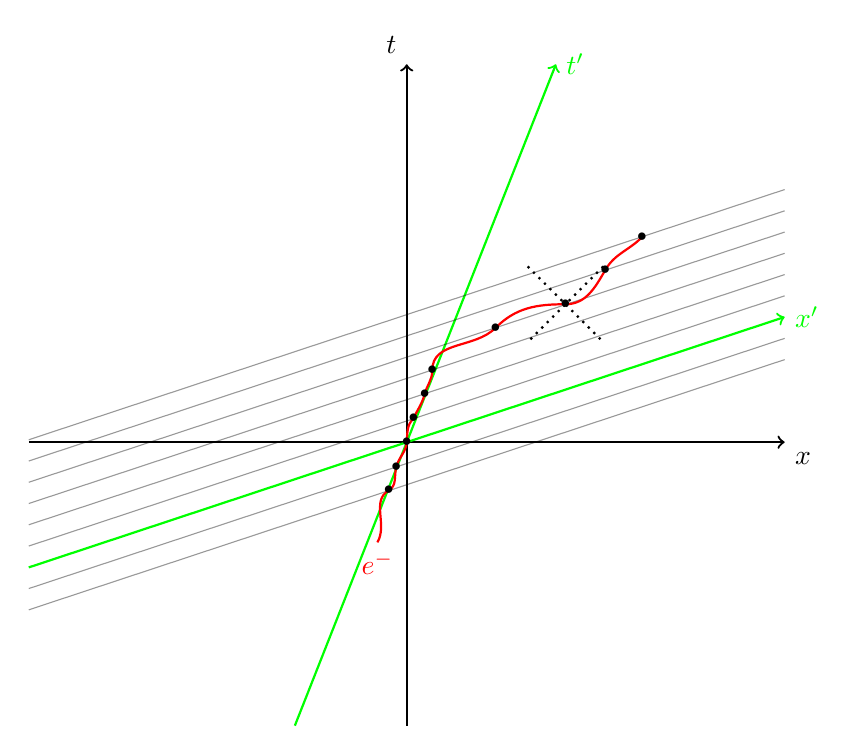
\begin{tikzpicture}[scale = 1.2]
                \draw[->, thick] (-4, 0) -- (4, 0) node[below right]{$x$};
                \draw[->, thick] (0, -3) -- (0, 4) node[above left]{$t$};
                %\draw[dotted, opacity = 0.9] (-3,-3) -- (3, 3);
                %\draw[dotted, opacity = 0.9] (-3,3) -- (3, -3);
                \draw[->, green, thick] (-1.184, -3) -- (1.579, 4) node[right]{$t'$};
                \draw[->, green, thick] (-4, -1.325) -- (4, 1.325) node[right]{$x'$};
                \draw[domain = -4:4, opacity = 0.4] plot(\x, {-0.225 + 0.331*\x});
                \draw[domain = -4:4, opacity = 0.4] plot(\x, {-0.45 + 0.331*\x});
                \draw[domain = -4:4, opacity = 0.4] plot(\x, {0.225 + 0.331*\x});
                \draw[domain = -4:4, opacity = 0.4] plot(\x, {0.45 + 0.331*\x});
                \draw[domain = -4:4, opacity = 0.4] plot(\x, {0.675 + 0.331*\x});
                \draw[domain = -4:4, opacity = 0.4] plot(\x, {0.9 + 0.331*\x});
                \draw[domain = -4:4, opacity = 0.4] plot(\x, {1.125 + 0.331*\x});
                \draw[domain = -4:4, opacity = 0.4] plot(\x, {1.35 + 0.331*\x});
                \draw[>=latex, red, thick] (-0.31, -1.06) node[below]{$e^-$} to[out = 60, in = 210] (-0.19, -0.51) node[black, scale = 0.7]{$\bullet$} to[out = 30, in = 255] (-0.11, -0.26) node[black, scale = 0.7]{$\bullet$} to[out = 75, in = 265] (0, 0) node[black, scale = 0.7]{$\bullet$} to[out = 85, in = 225] (0.07, 0.25) node[black, scale = 0.7]{$\bullet$} to[out = 65, in = 255] (0.19, 0.51) node[black, scale = 0.7]{$\bullet$} to[out = 75, in = 270] (0.27, 0.76) node[black, scale = 0.7]{$\bullet$} to[out = 90, in = 225] (0.94, 1.21) node[black, scale = 0.7]{$\bullet$} to[out = 45, in = 180] (1.68, 1.46) node[black, scale = 0.7]{$\bullet$} to[out = 0, in = 240] (2.1, 1.82) node[black, scale = 0.7]{$\bullet$} to[out = 60, in = 225] (2.49, 2.17) node[black, scale = 0.7]{$\bullet$};
                \draw[dotted,thick] (2.08,1.86) -- (1.28,1.06);
                \draw[dotted,thick] (1.28,1.86) -- (2.08,1.06);
            \end{tikzpicture}
            \caption{Ligne d'univers d'une particule supra-luminique}
            \end{figure}
            
            On peut alors faire un boost pour passer au référentiel $\R'$ afin de voir à quoi ressemble la ligne d'univers dans ce référentiel-là.
            
            \begin{figure}[H]
            \centering
            \begin{tikzpicture}[scale = 1.2]
                \draw[->, thick] (-4, 0) -- (4, 0) node[below right]{$x'$};
                \draw[->, thick] (0, -3) -- (0, 4) node[above left]{$t'$};
                \draw[domain = -4:4, opacity = 0.7] plot (\x, {0.35}) node[right]{$t'_1$};
                \draw[domain = -4:4, opacity = 0.7] plot (\x, {0.7});
                \draw[domain = -4:4, opacity = 0.7] plot (\x, {1.05});
                \draw[domain = -4:4, opacity = 0.7] plot (\x, {1.4});
                \draw[domain = -4:4, opacity = 0.7] plot (\x, {1.75}) node[right]{$t'_2$};
                \draw[>=latex, thick, red, ->] (-1, -2) node[below]{$e^-$} to[out = 70, in = 230] (0,0) ;
                \draw[>=latex, thick, red, ->] (0,0) to[out = 50, in = 180] (1.3, 1.75);  
                \draw[>=latex, thick, red, ->] (1.3, 1.75) to[out = 0, in = 180] (2.6, 0.35);
                \draw[>=latex, thick, red, ->] (2.6, 0.35) to[out = 0, in = 250] (3.9, 2.5);
            \end{tikzpicture}
            \caption{Ligne d'univers d'une particule supra-luminique}
            \end{figure}
            
            On voit bien que les lignes de simultanéité s'intersectionnent plusieurs fois avec la ligne d'univers ce qui veut dire qu'un observateur dans le référentiel $\R'$ voit plusieurs particules en même temps.\\
            
            La première chose importante est que l'on a supposé dès le départ que l'on était dans un cadre quantique. Ce genre de phénomène n'est pas observable dans un cadre purement relativiste. On voit que le nombre de particule n'est pas conservé. Si l'on voit une particule dans un certain référentiel, on peut en voir plusieurs dans un autre. Ceci suggère que le nombre de degré de liberté d'une théorie quantique relativiste devrait être infini. Les objets physiques qui ont cette caractéristiques sont les champs. On parle alors de théorie quantique des champs (QFT).\\
            
            La dernière conséquence du mariage de la relativité et de la mécanique quantique dont nous parlerons ici est le théorème spin-statistique. Ce théorème relie la nature du spin d'une particule (entier ou demi-entier) à sa distribution statistique (Bose-Einstein ou Fermi-Dirac). Les détails mathématiques de cette correspondance dépasse cependant le cadre de ces notes.